This section provides a benchmark and two case studies that showcase the effectiveness and applicability of our proposed approach. In the following Subsections, we investigate the properties and performance of the approach using streamed benchmark system data and signals from IoT devices in a microgrid system. The successful deployment demonstrates that this approach is suitable for existing process automation infrastructure.

The case studies were realized using Python 3.10.1 on a machine employing an 8-core Apple M1 CPU and 8 GB RAM.

\subsection{Benchmark}\label{AA:Benchmark}
In this subsection, we compare the proposed method with adaptive unsupervised detection methods without an interpretability layer. Two of the well-established methods, providing iterative learning capabilities over multivariate time-series data are One-Class Support Vector Machine (OC-SVM) and Half Spaced Trees (HS-Trees). Both methods represent the backbone of multiple state-of-the-art methods for cases of anomaly detection on dynamic system data, as we brief listed in Introduction \ref{par:validation}.

Comparison is conducted on real benchmarking data, annotated with labels of whether the observation was anomalous or normal. The dataset of Skoltech Anomaly Benchmark (SKAB) \cite{skab2020} is used for this purpose, as no established benchmarking multivariate data were found regarding energy storage systems. It represents a combination of experiments with the behavior of rotor imbalance as a subject to various functions introduced to control action as well as slow and sudden changes in the amount of water in the circuit. The system is described by 8 features and conveys slow and sudden drifts.

The data were preprocessed according to best practices for the given method, namely: standard scaling for OC-SVM, normalization for HS-Trees, while no scaling was required by our proposed method. Preprocessing is performed online as it would be in the production environment, with running mean and variance used in online standard scaler, while normalization employs running peak-to-peak distance. As stated in the employed library for the online machine learning river, such processing has no detrimental effect on performance in the long run (\cite{Montiel2021})

The optimal hyperparameters for both reference methods is found using Bayesian Optimization. Due to no further knowledge about the data generating process, and equity in benchmark, the hyperparameters of our proposed method were optimized using Bayesian Optimization as well. 20 steps of random exploration with 100 iterations of Bayesian Optimization were used, increasing default values set in the Bayesian Optimization library (\cite{Nogueira2014}).

The hyperparameters are optimized with F1 score as cost function first, to maximize both precision and recall on anomalous samples. Second, the hyperparameters are optimized with macro F1 score, as it considers performance on both anomalous samples as well as normal samples equally. Therefore, the performance is not indifferent towars type I. errors, false alarms due to wrong detection of normal data as anomalies.

As adaptation is required and anticipated within benchmark datasets, the performance is evaluated iteratively, similarly to the operation after deployment. The metric is updated with each new sample and its final value used to drive Bayesian Optimization. The performance is evaluated using the best performing model, found by Bayesian Optimization. The performance of the proposed method is evaluated on the same data.

Hyperparameter search ranges were specified regardless of the data domain. The ranges in both cases of OC-SVM and HS-Trees were centered around the default values of the library. The ranges for the proposed method were set arbitrarily wide, to allow the Bayesian Optimization to explore the space of hyperparameters. Values of quantile filter threshold were aligned with the threshold used in our proposed method. The ranges are provided in Table \ref{tab:hyperparam_ranges}.

\begin{table}[ht]
\centering
\caption{Hyperparameter Ranges for Detection Algorithms}
\label{tab:hyperparam_ranges}
\begin{tabular}{|l|l|c|c|}
\hline
\textbf{Algorithm} & \textbf{Hyperparameters} & \textbf{Default} & \textbf{Ranges} \\
\hline
AIM &
\begin{tabular}[c]{@{}l@{}}Threshold\\$t_e$\\$t_a$\\Grace Period\end{tabular} &
\begin{tabular}[c]{@{}c@{}}0.99735\\-\\$t_e$\\$t_e$\end{tabular} &
\begin{tabular}[c]{@{}c@{}}(0.85, 0.99993)\\(150, 500)\\(50, 1000)\\(50, 1000)\end{tabular} \\
\hline
OC-SVM &
\begin{tabular}[c]{@{}l@{}}Threshold\\Learning Rate\end{tabular} &
\begin{tabular}[c]{@{}c@{}}-\\0.01\end{tabular} &
\begin{tabular}[c]{@{}c@{}}(0.85, 0.99993)\\(0.005, 0.02)\end{tabular} \\
\hline
HS-Trees &
\begin{tabular}[c]{@{}l@{}}Threshold\\N Trees\\Max Height\\Window Size\end{tabular} &
\begin{tabular}[c]{@{}c@{}}-\\10\\8\\250\end{tabular} &
\begin{tabular}[c]{@{}c@{}}(0.85, 0.99993)\\(5, 15)\\(6, 10)\\(200, 300)\end{tabular} \\
\hline
\end{tabular}
\end{table}


The results are provided in Table \ref{tab:perf_comp}, evaluating F1 score, Recall and Precision. A value of 100\% at each metric represents a perfect detection. The latency represents the average computation time per sample of the pipeline including training and data preprocessing.

\begin{table}[htbp]
\begin{center}
\begin{tabular}{|l|c|c|c|c|}
    \hline
    \textbf{Algorithm} & F1 [$\%$] & Recall [$\%$] & Precision [$\%$] & Avg. Latency [ms] \\
    \hline
    AID & $\boldsymbol{48.70}$ & 49.90 & $\boldsymbol{47.56}$ & 1.55 \\
    \hline
    OC-SVM & 44.42 & $\boldsymbol{56.67}$ & 36.52 & 0.44 \\
    \hline
    HS-Trees & 34.10 & 32.57 & 35.77 & $\boldsymbol{0.21}$ \\
    \hline
\end{tabular}
\end{center}
\end{table}

The results in Table \ref{tab:perf_comp} suggest, that our algorithm provides slightly better performance than reference methods. Based on the Scoreboard for various algorithms on SKAB's Kaggle page, our iterative approach performs comparably to the evaluated batch-trained model. Such a model has all the training data available before prediction unlike ours, evaluating the metrics iteratively on a streamed dataset.

\subsection{Battery Energy Storage System (BESS)}\label{AA:BESS}
In the first case study, we verify our proposed method on BESS. The BESS reports measurements of State of Charge (SoC), supply/draw energy set-points, and inner temperature, at the top, middle, and bottom of the battery module. Tight battery cell temperature control is needed to optimize performance and maximize the battery's lifespan. Identifying anomalous events and removal of corrupted data might yield significant improvement in the process control level and increase the reliability and stability of the system.

The default sampling rate of the signal measurement is 1 minute. However, network communication of the IoT devices is prone to packet dropout, which results in unexpected non-uniformities in sampling. The data are normalized to the range $[0, 1$] to protect the sensitive business value. The proposed approach is deployed to the existing infrastructure of the system, allowing real-time detection and diagnosis of the system.

The industrial partner provided a physical model of the battery cell temperature, defined as follows:
\begin{align}
 \uis{T}{bat}{i+1} &= \uis{T}{bat}{i} + \ui{T}{s} (\ui{q}{fan} \ui{V}{b,max} \rho \ui{c}{p} (\ui{T}{out} - \uis{T}{bat}{i}) + \ui{V}{c,max}\ui{q}{circ.fan} \rho \ui{c}{p} \uis{T}{bat}{i} \nonumber \\
 &+ \ui{q}{circ.fan} (\ui{P}{cool} \ui{q}{cool} \ui{P}{heat} \ui{q}{heat}) + \ui{c}{scale} \ui{Q}{bat} + \ui{q}{inner fans} \\
 &- (\ui{V}{b,max} \ui{q}{fan} \ui{V}{c,max} \ui{q}{circ.fan}) \rho \ui{c}{p} \uis{T}{bat}{i}) / (\ui{m}{bat} \ui{c}{p,b}) \nonumber
\end{align}

When combined with an averaged measurement of battery cell temperature, we could compute the difference between real and predicted temperature. Such deviation can be useful in detecting unexpected patterns in temperature. Nevertheless, it may be inaccurate as the physical model is simplified and does not account for spatial aspects, like temperature gradients as well as different dynamic effects of charging and discharging on temperature. For instance, in Fig. \ref{fig:bess} mainly during the grace period we see, that the dynamics of cooling is not captured well, resulting in subtle positive difference between average cell temperature and the temperature predicted by the model. Therefore, the raw measured temperature is used as well.
The deviation between demanded power and delivered power was used to aid the identification of the state, as the increased difference might be related to other unexpected and novel patterns.

\begin{figure}[htbp]
\centerline{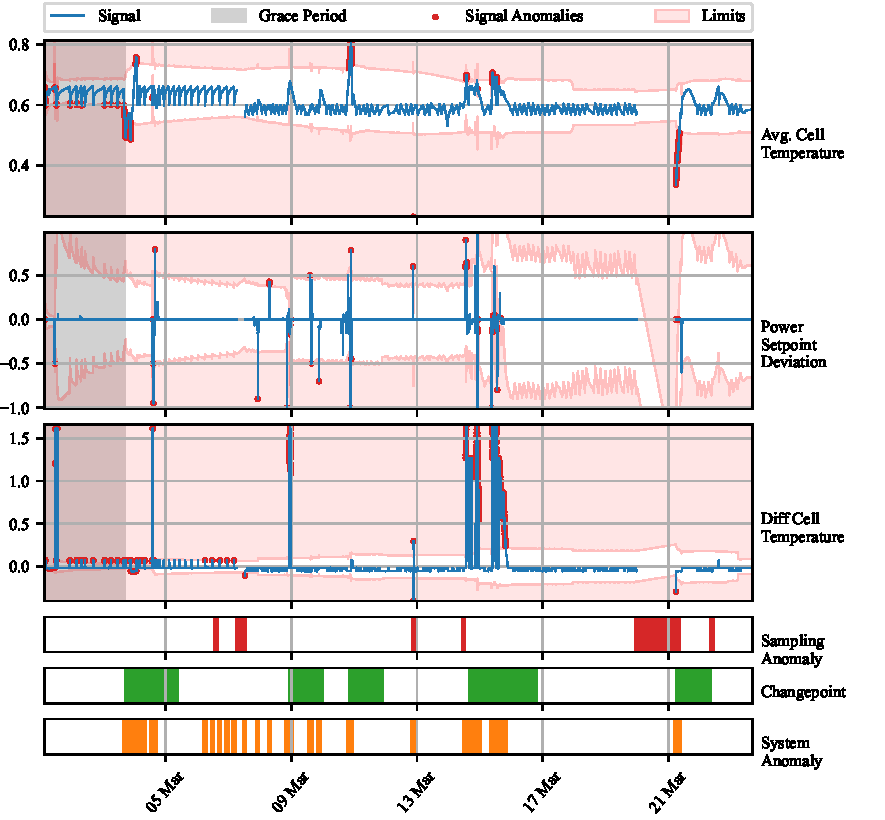
\includegraphics{figures/BESS_thresh.pdf}}
\caption{Time Series of BESS measurements (blue line) of process variables. The y-axis renders the values after the normalization of raw inputs. Root causes of anomalies are marked within specific signals as red dots. The light red area represents out-of-limits values for individual signals. Non-uniform sampling is marked as red bars. Green bars represent the times, at which changepoint was detected. All the signal anomalies are depicted as orange bars below the graph.}
\label{fig:bess}
\end{figure}

Fig. \ref{fig:bess} depicts the operation of the BESS over March 2022. Multiple events of anomalous behavior happened within this period, confirmed by the operators, that are observable through a sudden or significant shift in measurements in a given period. As the first step, the detection mechanism was initialized, following the provided guidelines for parameter selection in Subsection \ref{init}. The expiration period was set to $\ui{t}{e} = 7$ days, due to the weekly seasonality of human behavior impacting battery usage. The threshold was kept at default value $T = 0.99735$. A grace period, during which the model learns from both normal and anomalous data (though normal are expected, yet not required here), is shortened to 2.5 days to observe detectors reaction to the effect of tests performed on BESS happening on 3\textsuperscript{rd} day from deployment of the system.

As changepoint adaptation in presence of anomalies follows \eqref{eq:condition}, the tests on 3\textsuperscript{rd} day triggered adaptation, resulting in increased variance of distribution concerning Average Cell Temperature. The increased variance is observable in the light red area, loosening the region of normal operation.

The deployment and operation of the anomaly detection system demonstrate adaptation to changepoint on 7\textsuperscript{th} March 2022 that appeared due to the relocation of the battery storage system outdoors. The model adapted online due to 7 day window spcified by $\ui{t}{e}$. The sudden shift in environmental conditions, due to the transfer of the system to outside changed the dynamics of the system's temperature. The shift was subtle and the absolute temperature did not trigger alarm. On the other hand, However, new behavior was adopted by the AID framework within five days, reducing potential false alerts afterward, by observably shifting the conditional mean to lower temperatures. Perhaps more interesting are the alerted changepoint adaptation events.

Calibration of the BESS, usually observed as deviations of setpoint from real power demand and multiple peaks in temperature were captured as well.

The system identified 6 deviations in sampling, denoted by the red bars in Fig. \ref{fig:bess}. 4 anomalies with shorter duration represented packet loss. The prolonged anomaly was notified during the transfer of the battery pack. The longest dropout observed happened across 20\textsuperscript{th} March up to 21\textsuperscript{st}. Unexpectedly, the change point detection module triggered an alarm at the end of the loss, resulting in adaptation and a sharp shift in drawn limits for Power Setpoint Deviation. Red dots represent anomalies at the signal level given by equation \eqref{eq:anomaly_signal}. The dynamic signal limits are surpassed in one or multiple signals during the system's anomalies. The root cause isolation allows the pairing of anomalies with specific features. Conditional probability, against which the anomalies are evaluated allows consideration of signal relationships within individual limits.

\subsection{Kokam Battery Temperature Module}\label{AA:Kokam}
A second case study is concerned with monitoring temperature profiles of individual modules of battery pack deployed at end user. During the operation, a hardware fault of the cooling fan happened. Our industrial partner was interested in finding out, whether such an event could be captured by an anomaly detection system. The data for 12 modules, each coming with 6 channels of measurement were retrieved in 30-second sampling and processed in a streamed manner. We found it informative to compute the deviation of the observed value from the average of all the above-mentioned measurements.

Our anomaly detection system was, once again, initialized with an expiration period of 7 days. The grace period was shortened to 1 day. The threshold value was shifted to a 4 sigma value of 99.977\% to minimize the number of alarms.

In Figure \ref{fig:kokam} we observe 5 days of deviations between the observed temperature measured by channels of module 9 and the average temperature of all modules. After the grace period, we observe multiple system alarms raised by various channels. Until the noon of 22\textsuperscript{nd} August, they seem to be spread out randomly between individual channels. During the late evening of 22\textsuperscript{nd}, anomalies were reported by both channels 4 and 5 for a prolonged period, followed by an anomalous rise in temperature measured by channel 6 early in the morning on 23\textsuperscript{rd} August. The fan fault was observed approximately at 5 pm on 23\textsuperscript{rd} August. Our anomaly detection system instantly raised an alarm, notifying us of anomalous behavior reported by channels 1 - 3. The prolonged duration of the alarm triggered the changepoint alarm approximately 2 hours later. This resulted in a slightly faster adaptation of the system to the new operation under increased temperature. Surprisingly, the temperature decreased during the next day, notifying us of the fan being in operation for a brief period, to fail again 30 minutes later after the battery modules were cooled down to the previous setpoint. The anomaly detection system was triggered once again, although adaptation loosened the region of normal operation to allow itself to adapt. No significant anomalies in sampling were observed during the period.

\begin{figure}[htbp]
 \centerline{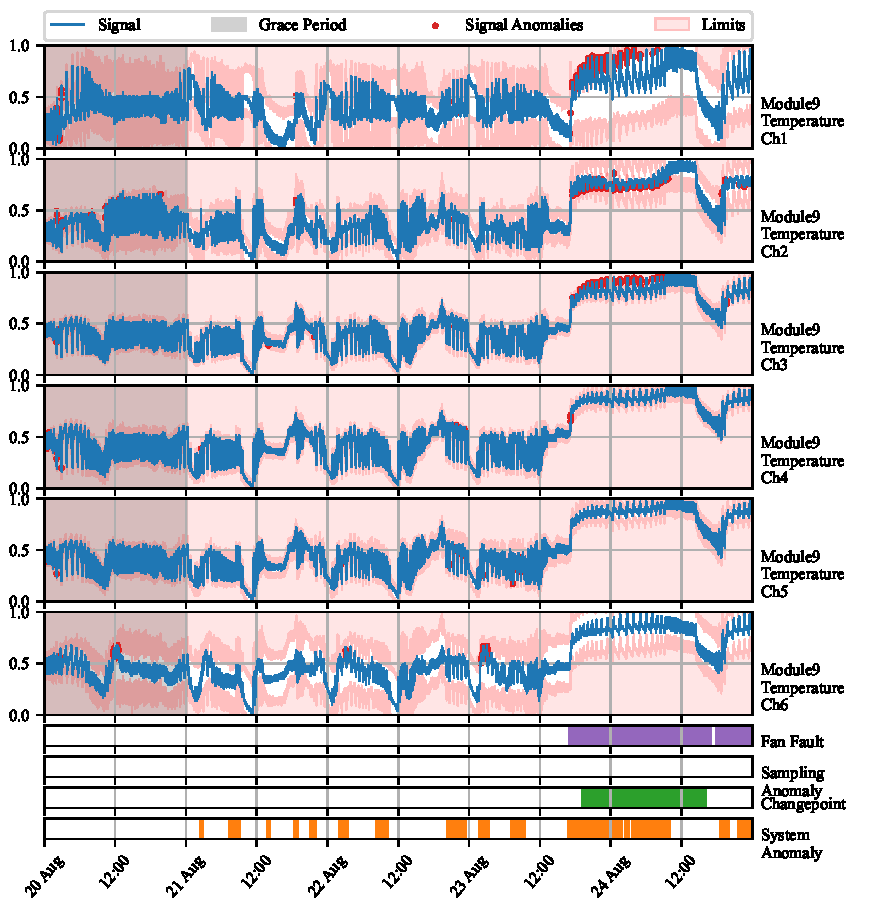
\includegraphics{figures/Kokam_thresh.pdf}}
 \caption{Time Series of battery module 9 measurements (blue line) of process variables. The y-axis renders the normalized deviations of temperature from average of all 12 modules. Signal anomalies are marked as red dots. The light red area represents out-of-limits values for individual signals. True fan faults are marked by purple bars. Green bars represent the times, at which changepoint was detected. All the signal anomalies are depicted as orange bars below the graph.}
 \label{fig:kokam}
\end{figure}
